\let\negmedspace\undefined
\let\negthickspace\undefined
\documentclass[journal]{IEEEtran}
\usepackage[a5paper, margin=10mm, onecolumn]{geometry}
%\usepackage{lmodern} % Ensure lmodern is loaded for pdflatex
\usepackage{tfrupee} % Include tfrupee package

\setlength{\headheight}{1cm} % Set the height of the header box
\setlength{\headsep}{0mm}  % Set the distance between the header box and the top of the text

\usepackage{gvv-book}
\usepackage{gvv}
\usepackage{cite}
\usepackage{amsmath,amssymb,amsfonts,amsthm}
\usepackage{algorithmic}
\usepackage{graphicx}
\usepackage{textcomp}
\usepackage{xcolor}
\usepackage{txfonts}
\usepackage{listings}
\usepackage{enumitem}
\usepackage{mathtools}
\usepackage{gensymb}
\usepackage{comment}
\usepackage[breaklinks=true]{hyperref}
\usepackage{tkz-euclide} 
\usepackage{listings}
% \usepackage{gvv}                                        
\def\inputGnumericTable{}                                 
\usepackage[latin1]{inputenc}                                
\usepackage{color}                                            
\usepackage{array}                                            
\usepackage{longtable}                                       
\usepackage{calc}                                             
\usepackage{multirow}                                         
\usepackage{hhline}                                           
\usepackage{ifthen}                                           
\usepackage{lscape}
\usepackage{tikz}
\usepackage{amsmath}

% Marks the beginning of the document
\begin{document} 

\bibliographystyle{IEEEtran}
\vspace{3cm}

\title{2012-GATE-ME-14-26}
\author{EE24BTECH11029- JANAGANI SHRETHAN REDDY}
\maketitle{}
%\newpage
\bigskip
\renewcommand{\thefigure}{\theenumi}
\renewcommand{\thetable}{\theenum}
\begin{enumerate}
    \item $\lim_{x\to 0}\brak{\frac{1-\cos{x}}{x^2}}$ is
    \begin{enumerate}
        \item $\frac{1}{4}$
        \item $\frac{1}{2}$
        \item $1$
        \item $2$
    \end{enumerate}
    \item A CNC vertical milling machine has to cut a straight slot of $10 mm$ width and $2 mm$ depth by a cutter of $10 mm$ diameter between points $\brak{0, 0}$ and $\brak{100, 100}$ on the $XY$ plane $\brak{dimensions in mm}$ The feed rate used for milling is $50$ $\frac{mm}{min}.$ Milling time for the slot $\brak{in seconds}$ is
    \begin{enumerate}
        \item $120$
        \item $170$
        \item $180$
        \item $240$
    \end{enumerate}
    \item A solid cylinder of diagram $100 mm$ and height $50 mm$ is forged between two frictionless flat dies to a height $25mm$. The percentage change in diameter is
    \begin{enumerate}
        \item $0$
        \item $2.07$
        \item $20.7$
        \item $41.4$
    \end{enumerate}
    \item The velocity triangles at inlet and exit of the rotor of a turbomachine are shown $V$ denotes blade velocity. subscripts $1$ and $2$ refer to inlet and outlet respectively.$V_2=W_1$ and $V_1=W_2$ then the degree of reaction is


\begin{tikzpicture}
    % Axes
    \draw[->] (2,0) -- (7,0) node[below ] {$U$};
    \draw[->] (0,3) -- (2,0) node[above right] {$W_1$};
    \draw[->] (0,3) -- (7,0) node[below right] {$V_1$};
    \draw[->] (9,3) -- (2,0) node[ above right] {$W_2$};
    \draw[->] (9,3) -- (7,0) node[below right] {$V_2$};
\end{tikzpicture}

    \begin{enumerate}
        \item $0$
        \item $1$
        \item $0.5$
        \item $0.25$
    \end{enumerate}
    \item Which one of the following configuration has the highest fin effectiveness?
    \begin{enumerate}
        \item Thin,closely spaced fins
        \item Thin,widely spaced fins
        \item Thick,widely spaced fins
        \item thick,closely spaced fins
    \end{enumerate}
    \item An ideal gas of mass $m$ and temperature $T_1$ undergoes a reversible isothermal process from an initial pressure $P_1$ to final pressure $P_2$. The heat loss during the process is $Q$. The entropy change $\triangle S$ of the gas is
    \begin{enumerate}
        \item $mR\ln\frac{P_2}{P_1}$
        \item $mR\ln\frac{P_1}{P_2}$
        \item $mR\ln\frac{P_2}{P_1}-\frac{Q}{_1}$
        \item $0$
    \end{enumerate}
    \item In the mechanism given below, if the angular velocity of the eccentric circular disc is $1\frac{rad}{s}$, the angular velocity $\frac{rad}{s}$ of the follower link for the instant shown in the figure is
    \begin{tikzpicture}
    % Draw the ground and pivot points
    \draw[thick] (0,0) -- (6,0); % Ground line
    \draw[fill=white] (0,0) circle (0.2); % Left pivot
    \draw[fill=white] (4.5,0) circle (0.2); % Right pivot
    
    % Draw the inclined beam
    \draw[thick] (0,0) -- (3.35,1.65); % Beam at an angle
     \draw[thick] (3.35,1.65) -- (3.2,1.85);
     \draw[thick] (3.2,1.85) -- (-0.55,0);
    % Draw the circle representing the rotating part
    \draw[thick] (4.5,0) circle (2); % Large circle with radius 25
    
    % Arrows and distances
    \draw[->] (4.5,0) -- ++(30:2) node[midway, above right] {25}; % Radius of the circle
    \draw[->] (4.5,-1.5) arc[start angle=-90, end angle=0, radius=0.5]; % Rotation arrow
    
    % Horizontal distances
    \draw[<->] (0,-0.5) -- (3.5,-0.5) node[midway, below] {45}; % Distance between pivots
    \draw[<->] (3.5,-0.5) -- (4,-0.5) node[midway, below] {5}; % Small horizontal distance

   \end{tikzpicture}
    \begin{enumerate}
        \item $0.05$
        \item $0.1$
        \item $5.0$
        \item $10.0$
    \end{enumerate}
    \item A circular solid disc of uniform thickness $20 mm$ radius $200mm$ and mass $20kg$, is used as a flywheel.If it rotates at $600 rpm$, the kinetic energy of the flywheel, in $joules$ is
    \begin{enumerate}
        \item $395$
        \item $790$
        \item $1580$
        \item $3160$
    \end{enumerate}
    \item A cantilever beam of length $L$ is subjected to moment $M$ at the free end. The moment of inertia of the beam cross section about the neutral axis $l$ and the Youngs modulus is $E$. The magnitude of the maximum deflection is
    \begin{enumerate}
        \item $\frac{ML^2}{2El}$
        \item $\frac{ML^2}{El}$
        \item $\frac{2Ml^2}{El}$
        \item $\frac{4ML^2}{El}$
    \end{enumerate}
    \item For a long slender column of uniform cross section, the ratio of critical buckling load for the case with both ends clamped to the case with both ends hinged is
    \begin{enumerate}
        \item $1$
        \item $2$
        \item $4$
        \item $8$
    \end{enumerate}
    \item At $x=0$, the function $f\brak{x}=x^3+1$ has
    \begin{enumerate}
        \item a mximum value
        \item a minimum value 
        \item a singularity
        \item a point of inflection
    \end{enumerate}
    \item For the spherical $x^2+y^2+z^2=1$, the unit outward normal vector at the point $\brak{\frac{1}{\sqrt{2}},\frac{1}{\sqrt{2}},0}$
    \begin{enumerate}
        \item $\frac{1}{\sqrt{2}}\Vec{i}+\frac{1}{\sqrt{2}}\Vec{j}$
        \item $\frac{1}{\sqrt{2}}\Vec{i}-\frac{1}{\sqrt{2}}\Vec{j}$
        \item $\Vec{
        k}$
        \item $\frac{1}{\sqrt{3}}\Vec{i}+\frac{1}{\sqrt{3}}\Vec{j}+\frac{1}{\sqrt{3}}\Vec{z}$
    \end{enumerate}
    CARRY TWO MARKS EACH
    \item The homogeneous state of stress for metal part undergoing plastic deformation is\\
    $T=\myvec{10&5&0\\5&20&0\\0&0&-10}$,\\
    where the stress component values are in $MPa$. Using Von Mises yield criterion, the value of estimated shear yield stress, in $MPa$
    \begin{enumerate}
        \item $9.50$
        \item $16.07$
        \item $28.52$
        \item $49.41$
    \end{enumerate}
\end{enumerate}
\end{document}T
